\section{Statistical analysis and results}

\subsection{Time evolution}
In order to determine the necessary amount of \textit{perturbation} $\rightarrow$ \textit{simulation} repetitions the time-evolution is shown for two different structures, namely $CS_4$ and $D_2$. they are tracked from ICs to final products with intermediate snapshots included as well ($10\_005$, $20\_005$ and $30\_005$ ). Here the analysis is based on the type $II_a$ sims. As can be seen from the figures, ten repetitions are sufficient as the structures at this point have become stable. Stable in this context means that continuing the \textit{perturbation} $\rightarrow$ \textit{simulation} experiment will not drastically change the profiles in any way (wrt. $\rho$, $\beta$ etc.). To see the effect of kick and flow independently figure 19 shows structure $CS_4$ at snapshot $19\_005$, then immediately after the next kick at snapshot $20\_000$ and finally after flow for a duration of one dynamical time at snapshot $20\_005$. In conclusion the flow is when changes to the structures become apparent but these changes were initiated at the kick so the two are co-dependent in order for this experiment to work. This teaches us about the scaling of both the size of the kicks and the number of dynamical times optimal for allowing the structures to settle into new stable configurations. As can be seen in the previous section under 
Controlled sim. II, dynamical times were set to either 1, 3 or 5. Kicks were either $5\%$, $20\%$ or $30\%$.

\begin{figure}[!htbp]
\centering
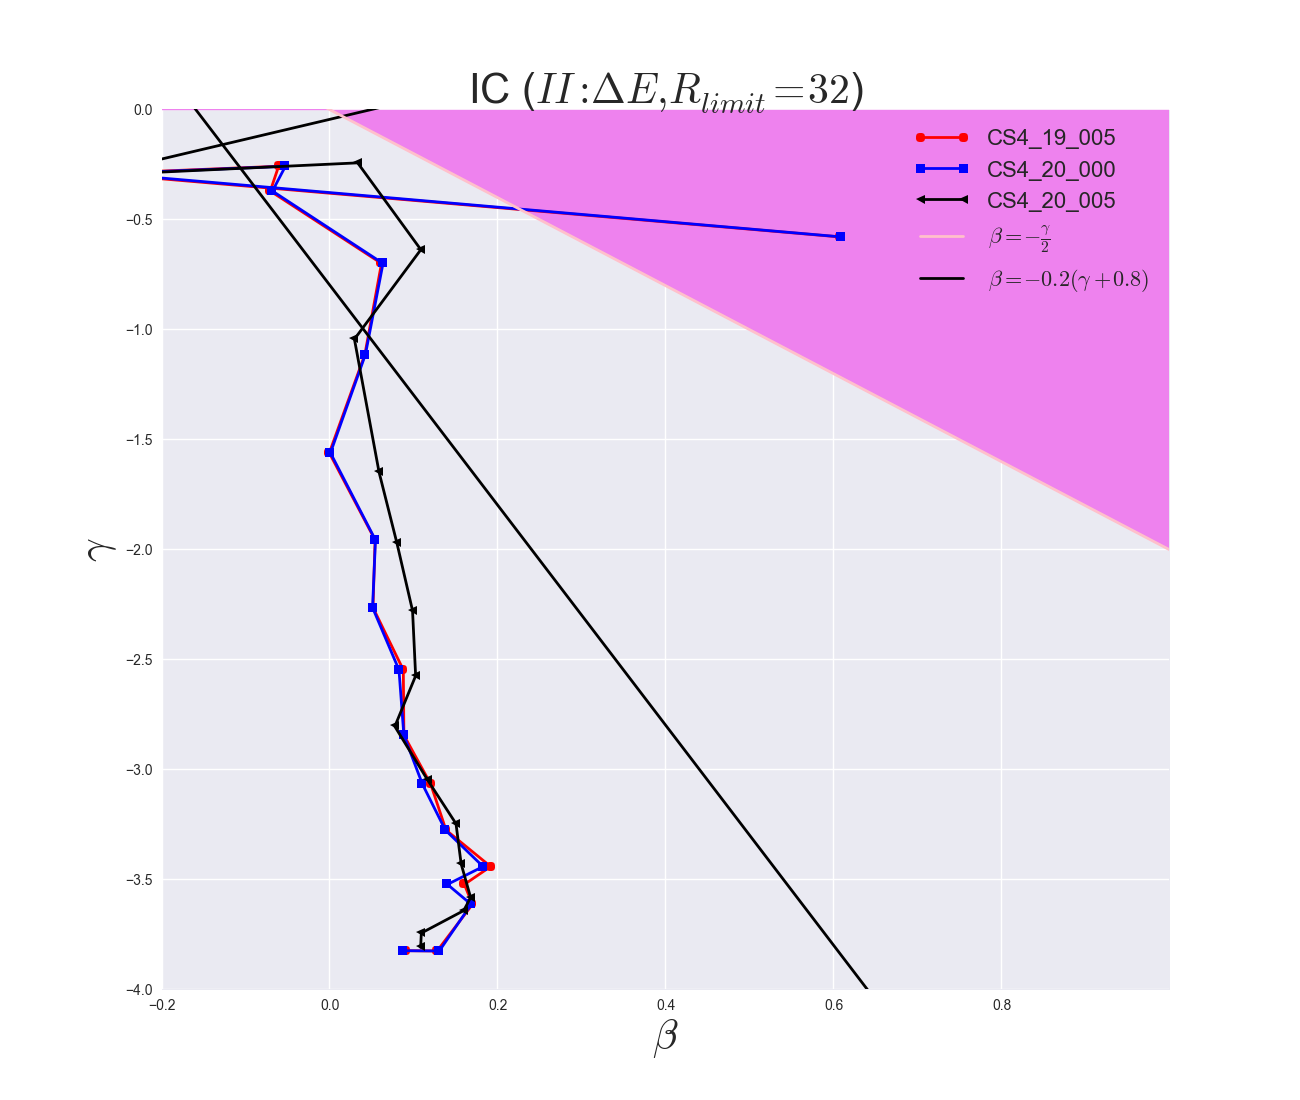
\includegraphics[width=1.0\linewidth]{img/beta_vs_gamma_CS4_Time_evolution_Rlimit32.png}
\caption{$\gamma$ vs. $\beta$ for 19$\_$005, 20$\_$000 and 20$\_$005 of sim. IIa of structure CS4.
Also shown is the linear $\beta$-$\gamma$ relation discovered by Hansen and Moore (2006) for comparison. The pink upper right area is found to be an unstable region by An and Evans (2006). This figure shows us the impact of perturbation and flow independently. Whereas the kick does not change the structure significantly on this type of plot, the subsequent simulation produces substantial alteration. It is thus the combination of both which serves to drive structures towards new equilibria just the same way as violent relaxation and phase mixing have synergestic effects on galaxies during late stages of mergers.}
\label{fig:test}
\end{figure}

\begin{figure}[!htbp]
\centering
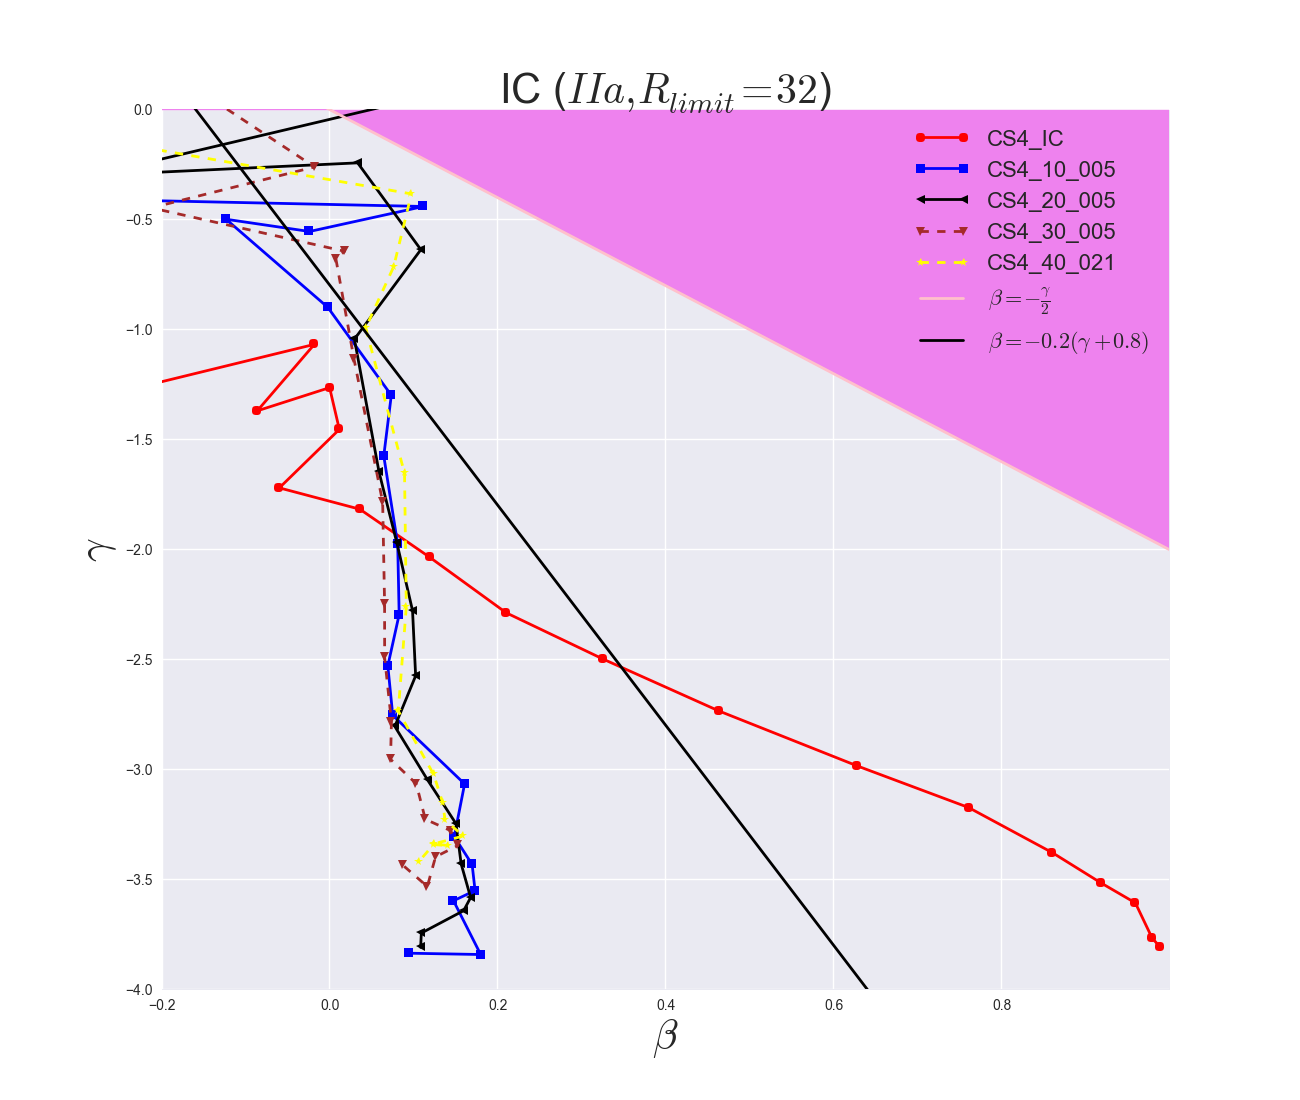
\includegraphics[width=1.0\linewidth]{img/beta_vs_gamma_CS4_Time_evolution_Rlimit32_IIa.png}
\caption{$\gamma$ vs. $\beta$ for IC, 10, 20, 30 and final product of sim. IIa of structure CS4. Also shown is the linear $\beta$-$\gamma$ relation discovered by Hansen and Moore (2006) for comparison. The pink upper right area is found to be an unstable region by An and Evans (2006).
Already after 10 runs the attractor state is present where $\beta = 0.1$ in the outer region.}
\label{fig:test}
\end{figure}

\begin{figure}[!htbp]
\centering
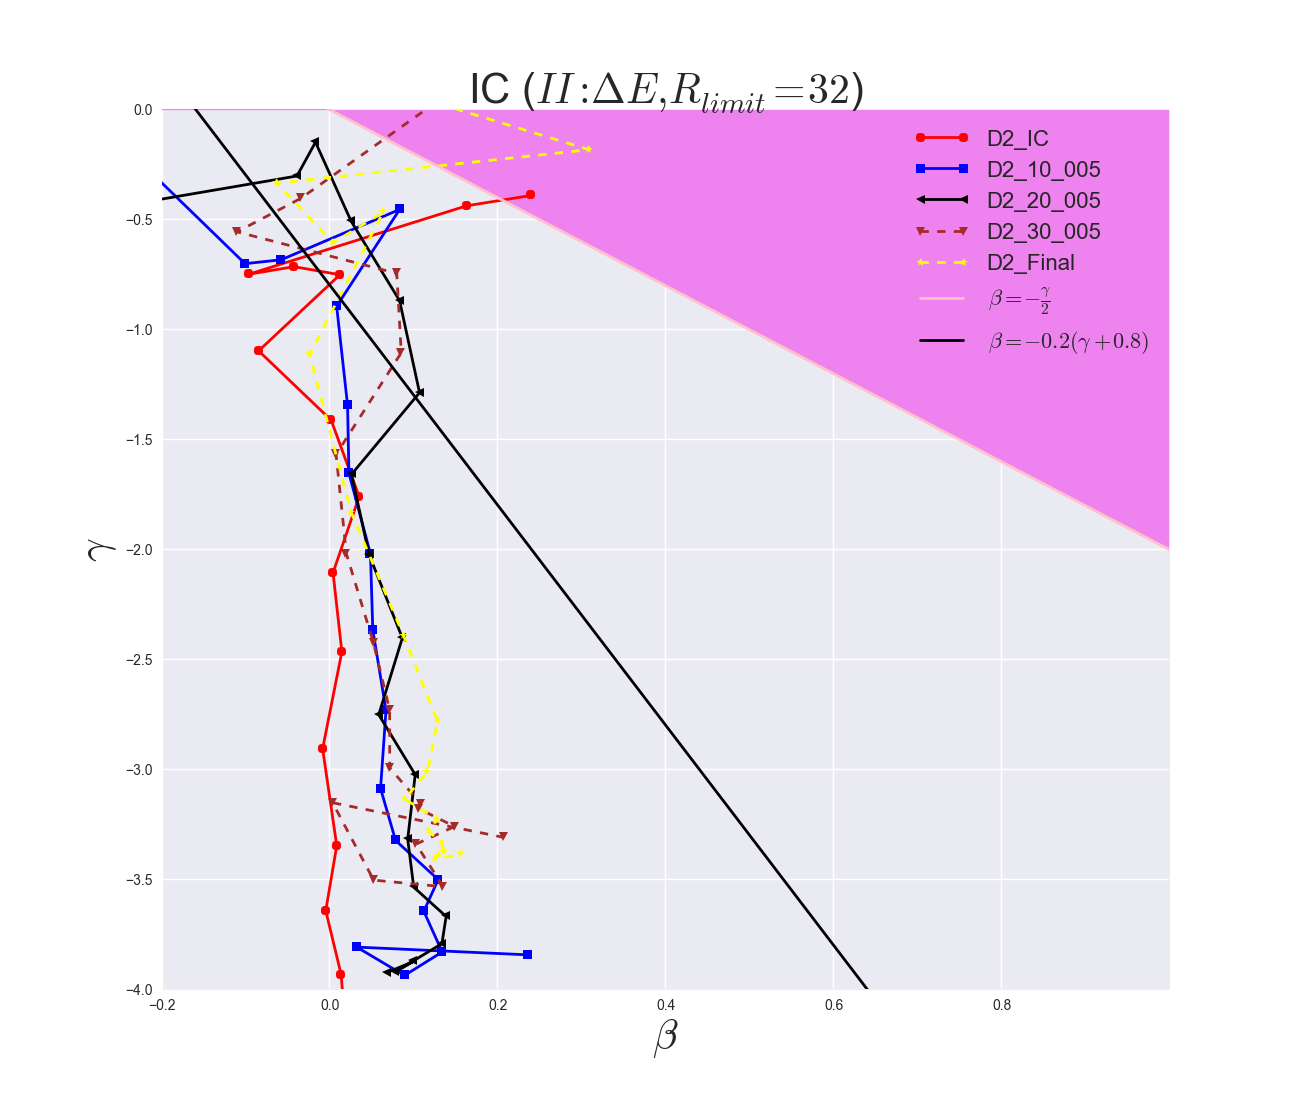
\includegraphics[width=1.0\linewidth]{img/beta_vs_gamma_D2_Time_evolution_Rlimit32.png}
\caption{$\gamma$ vs. $\beta$ for IC, 10, 20, 30 and final product of sim. IIa of structure D2. Also shown is the linear $\beta$-$\gamma$ relation discovered by Hansen and Moore (2006) for comparison. The pink upper right area is found to be an unstable region by An and Evans (2006).
Already after 10 runs the attractor state is present where $\beta = 0.1$ in the outer region.}
\label{fig:test}
\end{figure}

\subsection{Selection of radial domains}
To study local properties of halos more clearly, four distinct regions of structures are plucked out. Radii corresponding to the four $\gamma$-values -1.5, -2.0, -2.5 and -3.0 are taken as central values in bins spanning a with where excactly $10^4$ particles are included. The result of this localized analysis is that the central, majority of particles in structures are well behaved for all sim. in this work (I, $II_a$, $II_b$, $II_c$ and $II_d$) but that the very inner parts are fluctuating due to the approach of gravitational softening length and similarly the very outer parts fluctuates due to insufficient simulation time (the dynamical time at large radii can be very large). See figure 34.


\begin{figure}[!htbp]
\centering
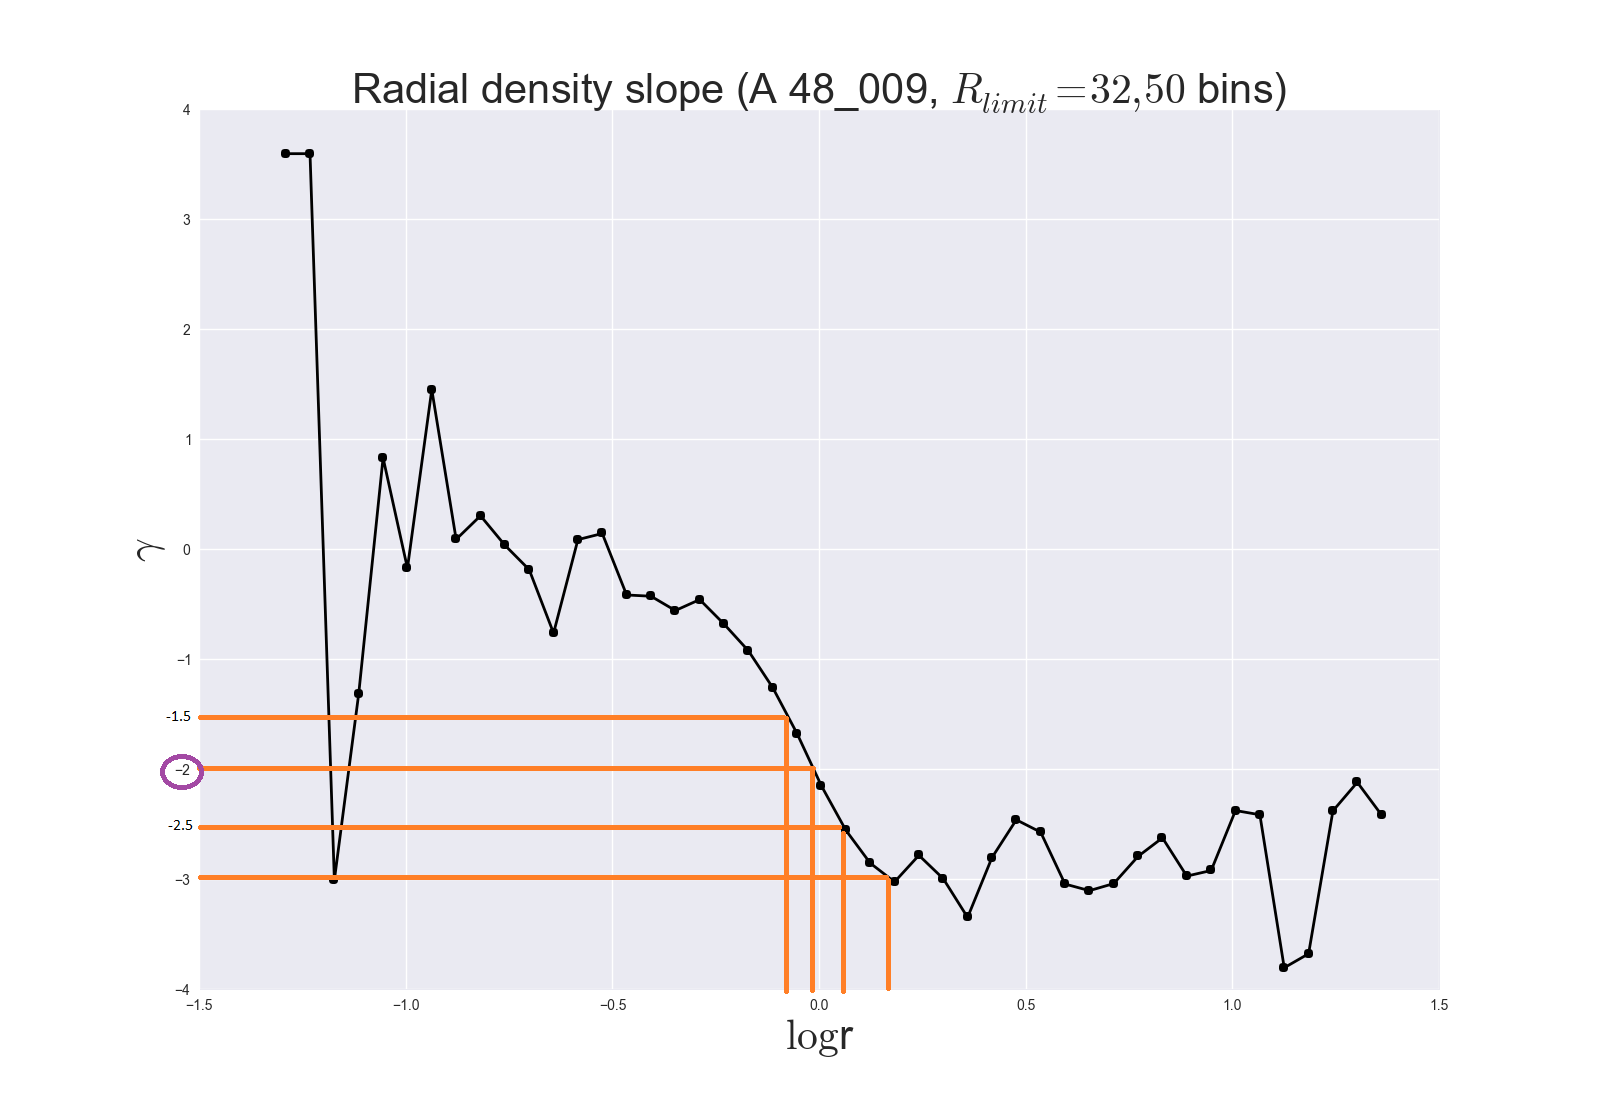
\includegraphics[width=1.0\linewidth]{img/A_48_009_gamma_logr_I_R32.png}
\caption{$\gamma$ vs. $\log r$ for final product of sim. I of structure A (48$\_$009).
The structure is initially cut off at a radius of $R_{lim} = 32\cdot r_s$ (corresponding to the $log_{10}$ value of 1.5) 
Four $\gamma$-values of interest are chosen (indicated by the horizontal orange lines):
$\gamma = -1.5$, -2, -2.5 and -3,
which correspond to four different $\log$ r values, namely
$\log (r_{-1.5})$, $\log (r_{-2})$, $\log (r_{-2.5})$ and $\log (r_{-3})$ respectively (indicated by the vertical orange lines).
In particular $\gamma = -2$ (marked by a purple ring) is of interest for Hernquist structures as its corresponding $\log (r_{-2})$-value indicates the point where the density slope takes on its mean value.
$r_{-2}$ thus introduces a natural length unit which makes comparison between different Hernquist structures with for example different number of particles more meaningful.}
\label{fig:test}
\end{figure}

\subsection{Cuts and range of trust}
Figure 35-37 shows examples of how cuts are chosen.
Noise in inner and outer regions determines the cutting points for inner and outer cuts
and these cuts are performed for both the $\gamma$ vs. $\log r$ plots, the $\kappa$ vs. $\log r$ plots and the $\beta$ vs. $\log r$ plots. Comparing these three parameter plots with cuts found for each,
the most conservative overall inner and outer cuts are determined and applied to that particular structure. This is done for all structures, and the attractor plot (final products after sim. I plotted as $\gamma + \kappa$ vs. $\beta$) can then be seen for the stable regions of all structures undergoing sim. I.
 This principle is then applied to all simulations (I, $II_a$, $II_b$, $II_c$ and $II_d$). 

\begin{figure}[!htbp]
\centering
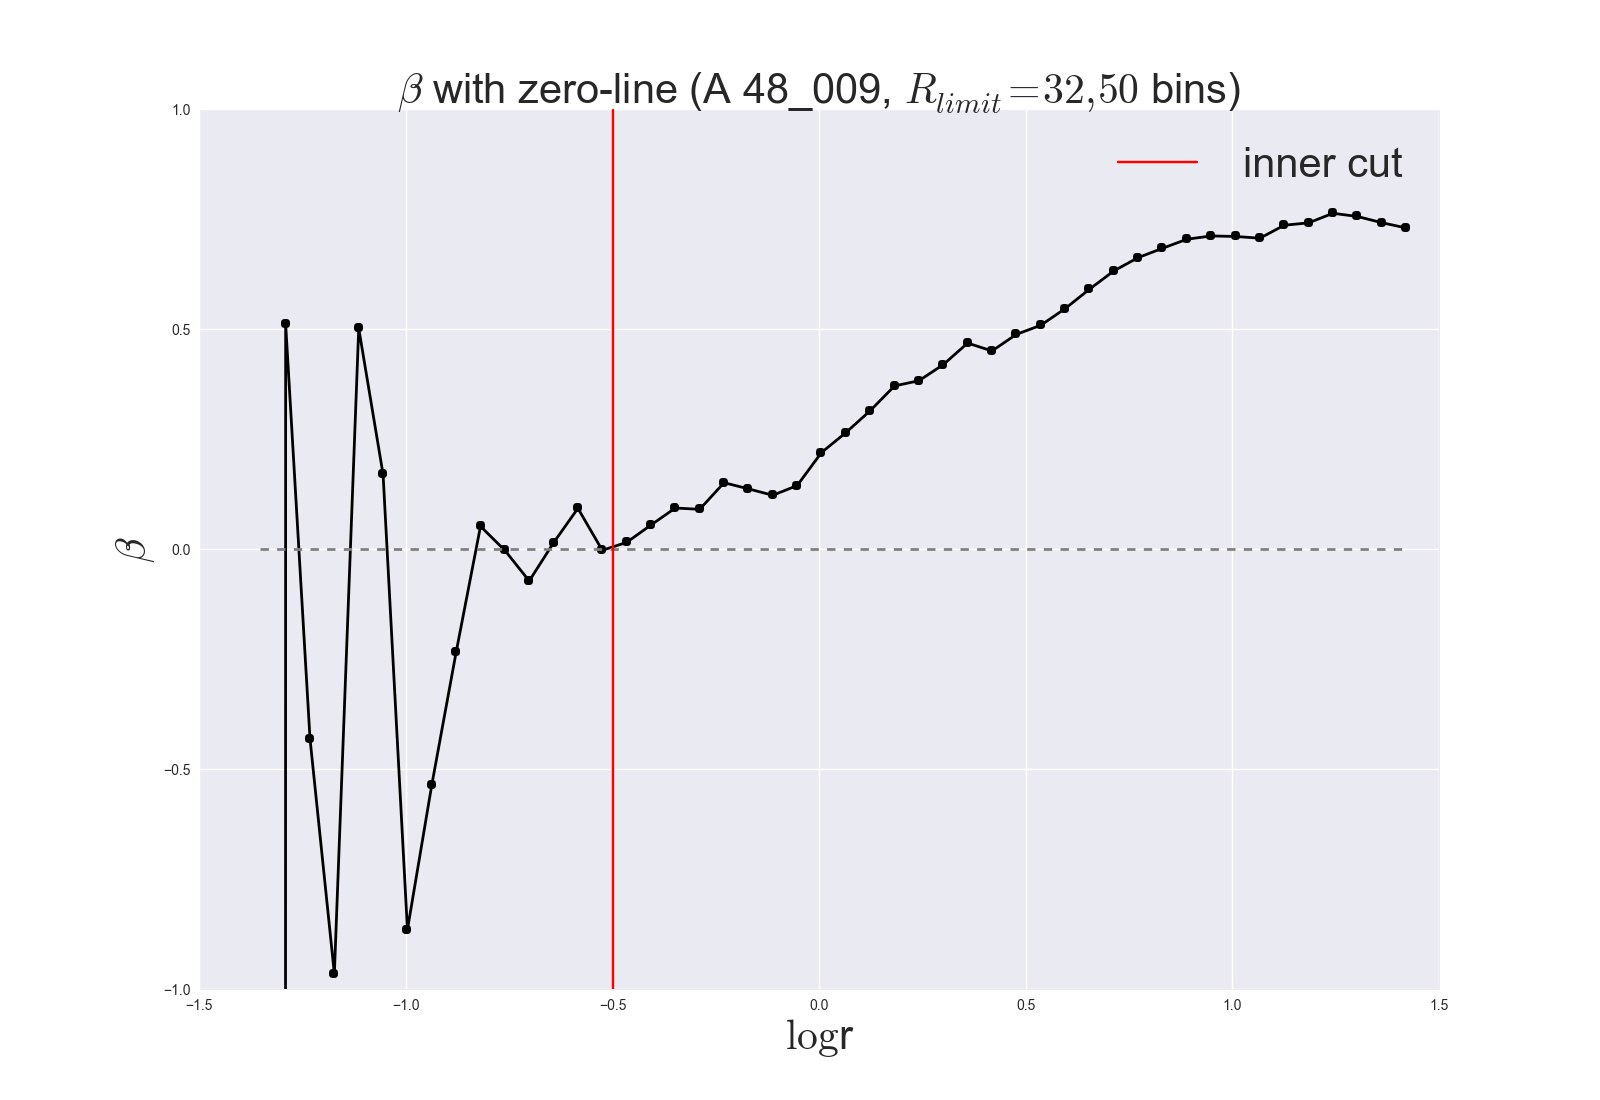
\includegraphics[width=1.0\linewidth]{img/A_48_009_beta_logr_I_R32_cuts.png}
\caption{$\beta$ vs. $\log r$ for final product of sim. I of structure A (48$\_$009).
The structure is initially cut off at a radius of $R_{lim} = 32\cdot r_s$ (corresponding to the $log_{10}$ value of 1.5) 
after which one additional (inner) cut is applied to the $\beta$-profile.
This inner cut (shown in red and located at $\log r = -0.5$) gets rid of Poisson noise due to the discrete nature of the N-body code, 
The remaining points on the $\beta$-profile thus only exist in the $\log r $ interval of [-0.5,1.5], namely the points with numbers [16;48].}
\label{fig:test}
\end{figure}

\begin{figure}[!htbp]
\centering
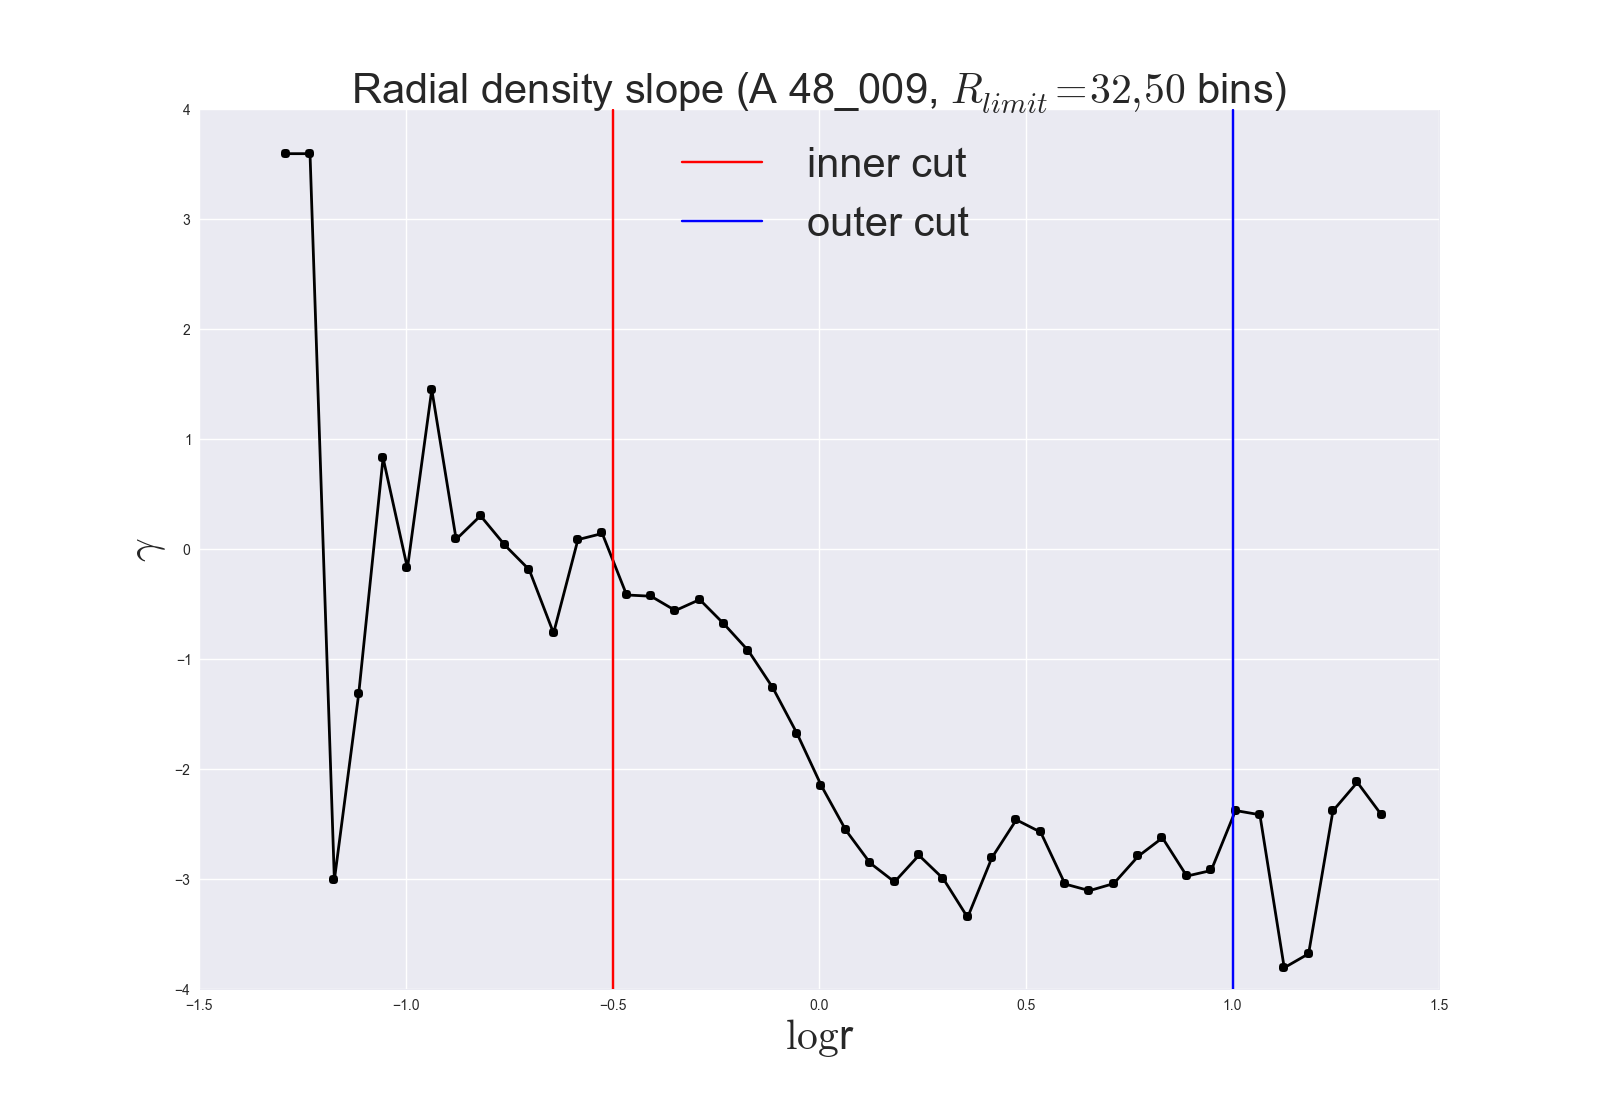
\includegraphics[width=1.0\linewidth]{img/A_48_009_gamma_logr_I_R32_cuts.png}
\caption{$\gamma$ vs. $\log r$ for final product of sim. I of structure A (48$\_$009).
The structure is initially cut off at a radius of $R_{lim} = 32\cdot r_s$ (corresponding to the $log_{10}$ value of 1.5) 
after which two further cuts are applied to the $\gamma$-profile.
The inner cut (shown in red and located at $\log r = -0.5$) gets rid of Poisson noise due to the discrete nature of the N-body code, 
whereas the outer cut (shown in blue and located at $\log r = 1.0$) removes points far away from the halo center, where the particles have not yet had sufficient time to reach a stable equilibrium.
The remaining points on the $\gamma$-profile thus only exist in the $\log r $ interval of [-0.5,1.0], namely the points with numbers [15;39].}
\label{fig:test}
\end{figure}

\begin{figure}[!htbp]
\centering
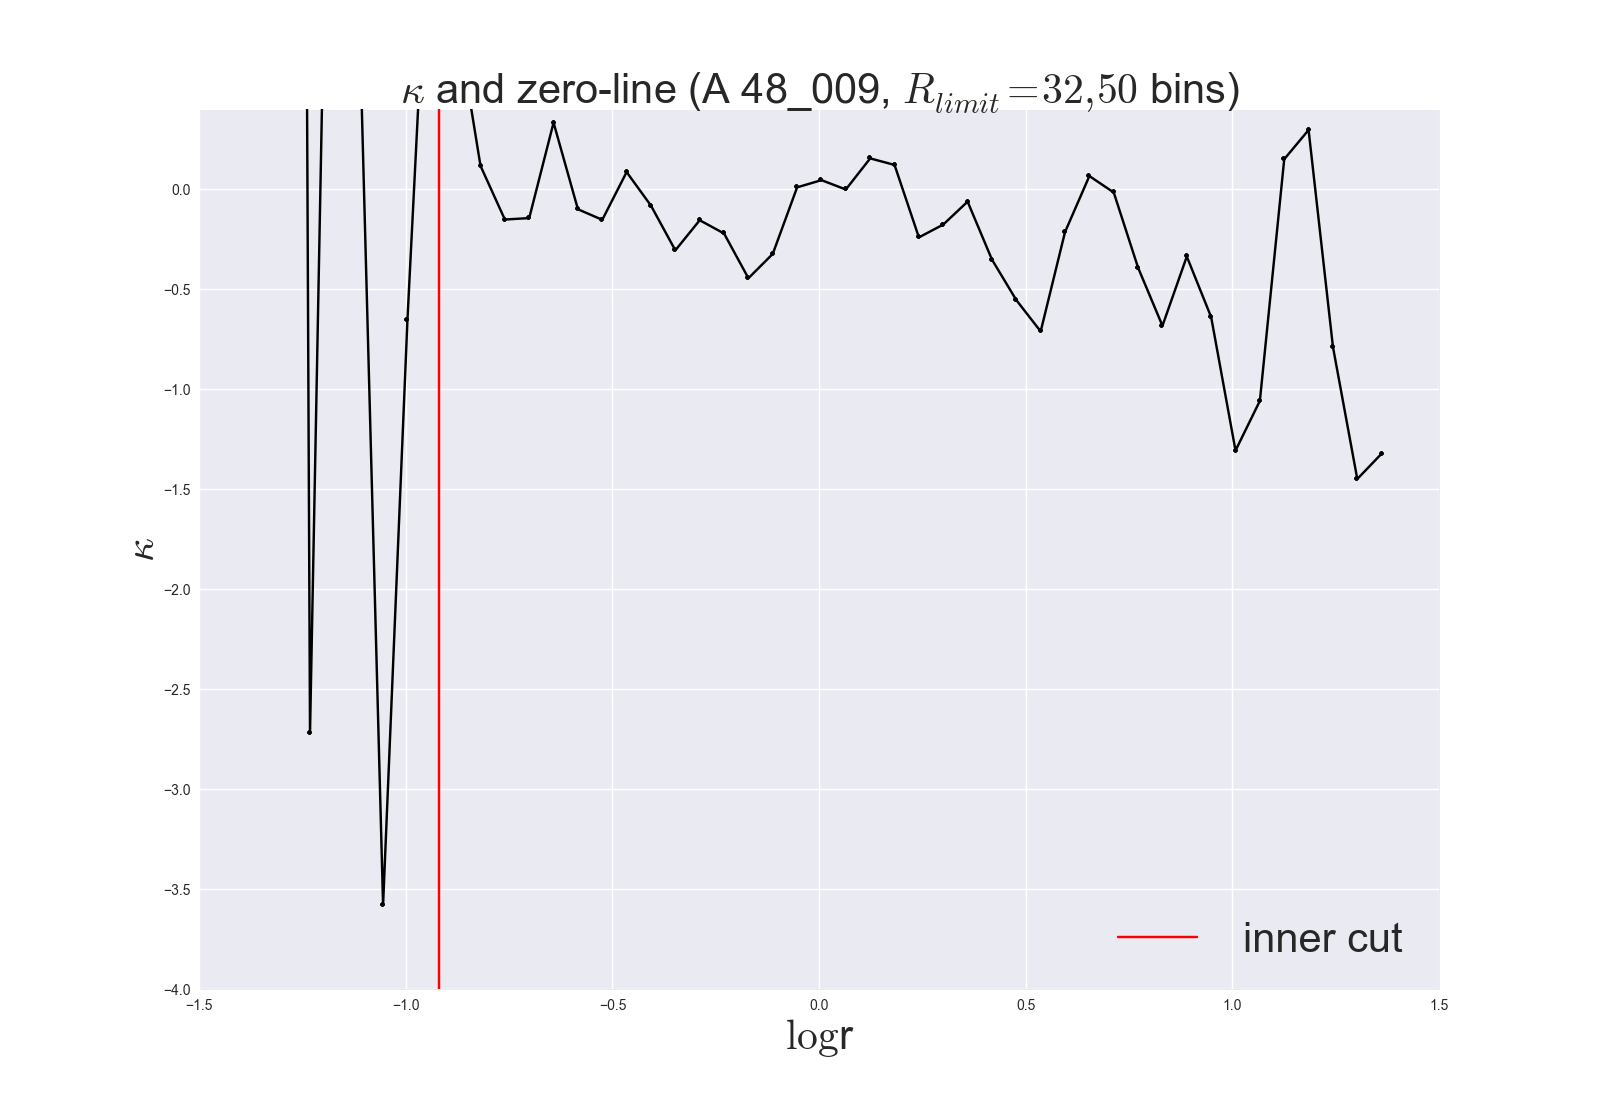
\includegraphics[width=1.0\linewidth]{img/A_48_009_kappa_logr_I_R32_cuts.png}
\caption{$\kappa$ vs. $\log r$ for final product of sim. I of structure A (48$\_$009).
The structure is initially cut off at a radius of $R_{lim} = 32\cdot r_s$ (corresponding to the $log_{10}$ value of 1.5) 
after which one additional (inner) cut is applied to the $\kappa$-profile.
This inner cut (shown in red and located at $\log r \approx -0.9$) gets rid of Poisson noise due to the discrete nature of the N-body code, 
The remaining points on the $\kappa$-profile thus only exist in the $\log r $ interval of [-0.9,1.5], namely the points with numbers [8;46].}
\label{fig:test}
\end{figure}

\begin{figure}[!htbp]
\centering
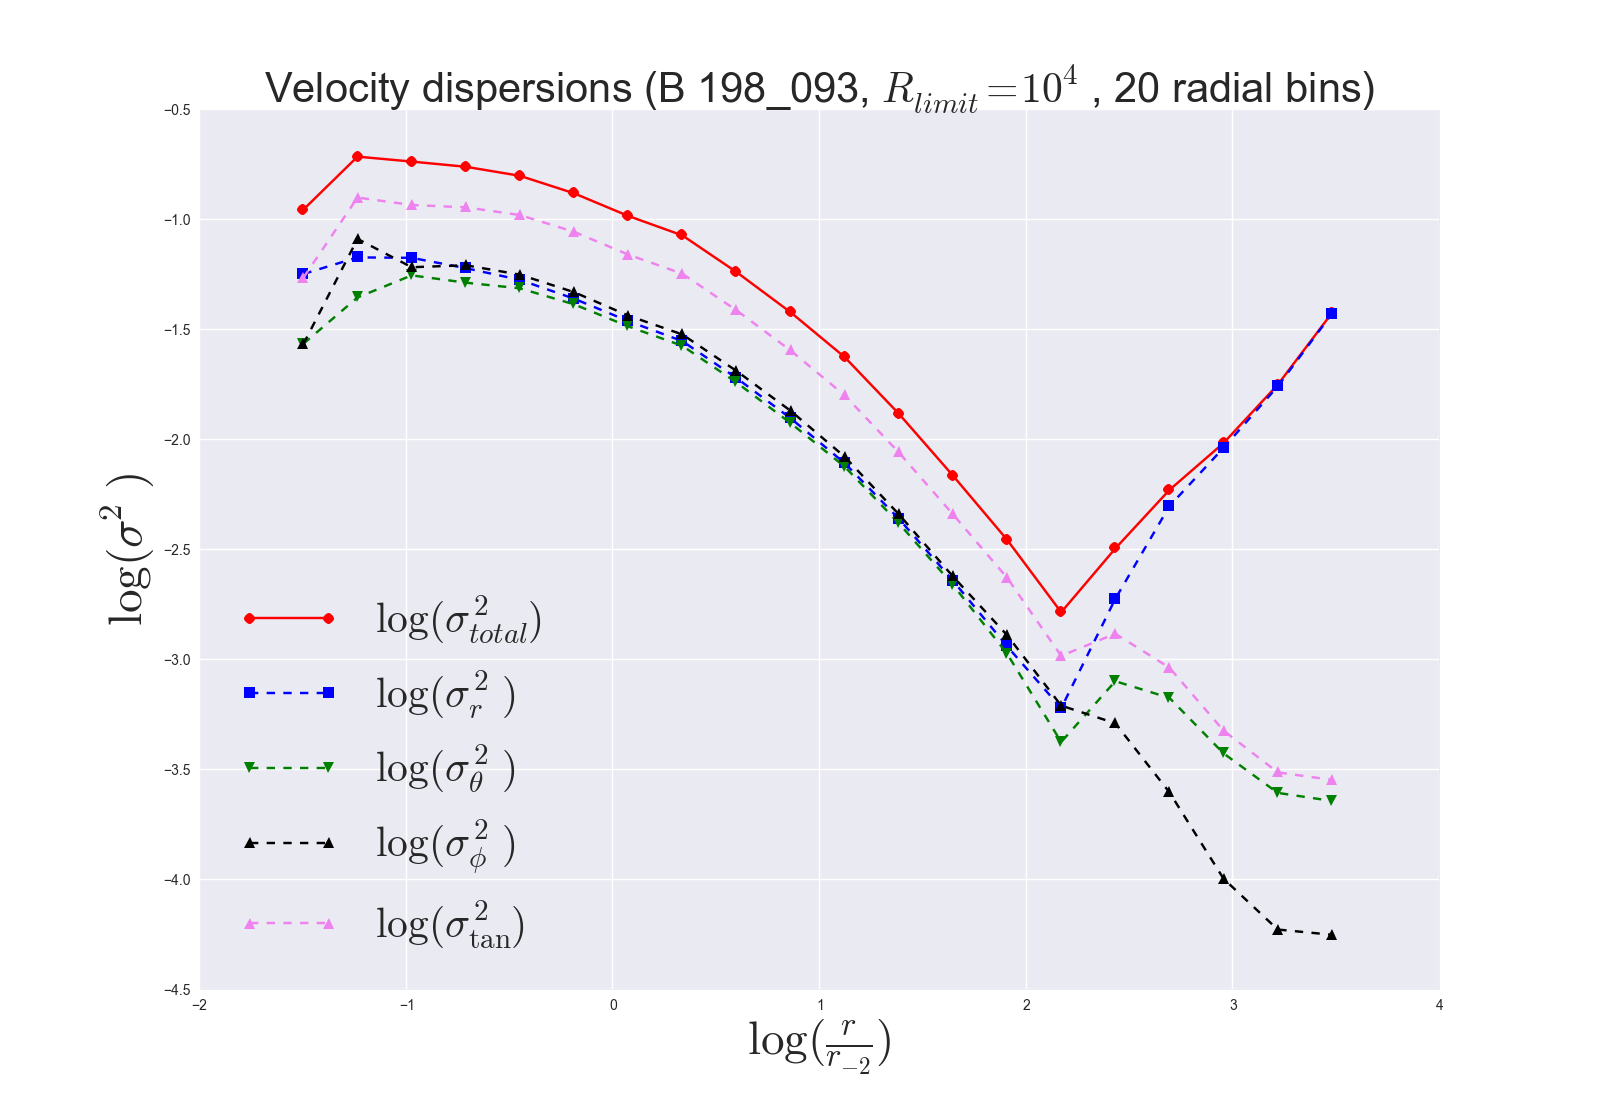
\includegraphics[width=1.0\linewidth]{img/B_198_093_sigma_r_2.png}
\caption{$\log (\sigma^2)$ vs. $\log (\frac{r}{r_{-2}})$ for one of the final products (198$\_$093) of Sim. I for structure B. 
20 bins logarithmic in radius is used and the structure is cut off at radius $R_{limit} = 10^4$ in arbitrary units of radius.
$\sigma^2$ is calculated as $\sigma^2 = \frac{1}{n}\cdot \sum\limits_{i=1}^n (v_i - <v>)^2$ inside each bin, where n is the number of particles inside a particular bin and <v> is the average velocity inside this bin.
For the inner and middle part of this structure the total dispersion is much greater than the 
radial dispersion and greater than the tangential dispersion, but at large radii (from $\log (\frac{r}{r_{-2}}) \approx 2.3$) it can be seen that the radial part starts to dominate over the tangential part and finally almost the entire total dispersion comes from the radial dispersion whereas the tangential dispersion in the outer part is almost negligible.}
\label{fig:test}
\end{figure}

\subsection{Unstable OM models}
OM models with HQ density profiles are unstable when $r_a < 1.33$, since this will cause radial orbit instability (ROI), creating a central bar structure. Several such structures are created ($C_1 \rightarrow C_6$) plus an additional OM structure with inner and outer density slopes (0,-5), ($D_1$). None of them lands on an attractor in the Jeans parameter space. This is in agreement with [8]. See the previous section 'Overview of structures' for more details concerning these profiles.

\textbf{We have highlighted various features from the simulations in this section and the next part summarizes the most important results for the entire project.}